\section{Đề ôn thi giữa kỳ 2 toán 11}
\subsection{Phần trắc nghiệm}
Câu trắc nghiệm nhiều phương án lựa chọn. Học sinh trả lời từ
câu 1 đến câu 12. Mỗi câu hỏi học sinh \textit{chỉ chọn một} phương án.
\Opensolutionfile{ans}[Ans/Dapan]

\hienthiloigiaiex
%%%=============EX_1=============%%%
\begin{ex}%[1D6N1-1]%[Dự án đề kiểm tra Toán khối 11 GHKII NH23-24-Dot 2-Nguyễn Vương Hiển]%[Deso3-Phan Nhật Linh]
	Cho $a$ là số thực dương khác $1$. Giá trị của biểu thức $P=a^{\tfrac{2}{3}}\cdot\sqrt{a}$ bằng
	\choice
	{$a^3$}
	{$a^{\tfrac{2}{3}}$}
	{\True $a^{\tfrac{7}{6}}$}
	{$a^{\tfrac{5}{6}}$}
	\loigiai{
		Ta có $P=a^{\tfrac{2}{3}}\cdot\sqrt{a}=a^{\tfrac{2}{3}}\cdot a^{\tfrac{1}{2}}=a^{\tfrac{7}{6}}$. 
	}
\end{ex}
\begin{ex}%[1D6N2-1]%[Dự án đề kiểm tra Toán khối 11 GHKII NH23-24-Dot 2-Nguyễn Vương Hiển]%[Deso3-Phan Nhật Linh]
	Với số thực dương $a$ bất kì, giá trị của $\log_22a$ bằng
	\choice
	{\True $1+\log_2a$}
	{$2+\log_2a$}
	{$4+\log_2a$}
	{$2\log_2a$}
	\loigiai{
		Ta có $\log_22a=\log_22+\log_2a=1+\log_2a$.		
	}
\end{ex}
\begin{ex}%[1D6N1-3]%[Dự án đề kiểm tra Toán khối 11 GHKII NH23-24-Dot 2-Nguyễn Vương Hiển]%[Deso3-Phan Nhật Linh]
	Tập xác định của hàm số $y=(x^2-2x-3)^{-4}$ là
	\choice
	{$\mathscr{D}=\mathbb{R}$}
	{\True $\mathscr{D}=\mathbb{R}\setminus\{-1;3\}$}
	{$\mathscr{D}=(-\infty;-1)\cup(3;+\infty)$}
	{$\mathscr{D}=(-1;3)$}
	\loigiai{
		Điều kiện: $x^2-2x-3\ne0\Leftrightarrow\heva{&x\ne-1\\&x\ne3.}$\\
		Vậy tập xác định của hàm số $y=(x^2-2x-3)^{-4}$ là $\mathscr{D}=\mathbb{R}\setminus\{-1;3\}$.		
	}
\end{ex}
\begin{ex}%[1D6N2-1]%[Dự án đề kiểm tra Toán khối 11 GHKII NH23-24-Dot 2-Nguyễn Vương Hiển]%[Deso3-Phan Nhật Linh]
	Cho $a$ là số thực dương khác $1$. Giá trị của biểu thức $\log_a a^{\tfrac{1}{3}}$ bằng
	\choice
	{$-\dfrac{1}{3}$}
	{\True $\dfrac{1}{3}$}
	{$3$}
	{$-3$}
	\loigiai{
		Ta có $\log_a a^{\tfrac{1}{3}}=\dfrac{1}{3}$.		
	}
\end{ex}
\begin{ex}%[1D6H3-1]%[Dự án đề kiểm tra Toán khối 11 GHKII NH23-24-Dot 2-Nguyễn Vương Hiển]%[Deso3-Phan Nhật Linh]
	\immini{
		Cho các hàm số $y=a^x$, $y=\log_b x$, $y=x^c$ có đồ thị như hình vẽ. Khẳng định nào sau đây là đúng.
		\choice 
		{$0<c<1<a<b$}
		{\True $c<0<a<1<b$}
		{$c<0<a<b<1$}
		{$0<c<a<b<1$}
	}{
		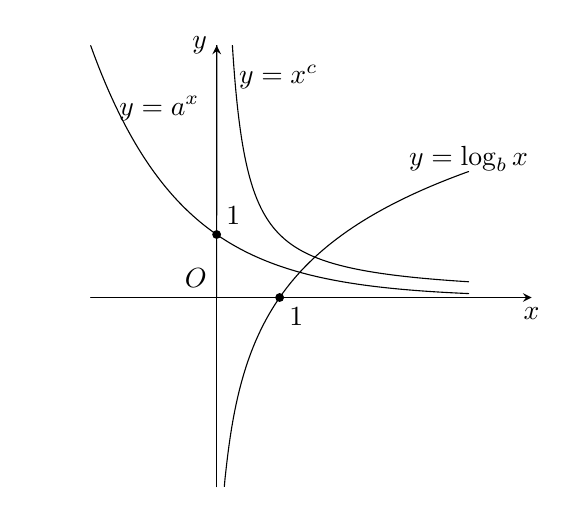
\begin{tikzpicture}[>=stealth,scale=0.8, line join=round, line cap=round]
			\draw[->] (-2,0)--(5,0) node [below]{$x$};
			\draw[->] (0,-3)--(0,4) node [left]{$y$};
			\node at (0,0) [above left]{$O$};
			\clip (-3,-3) rectangle (5,4); 
			\fill[black] (0,1) circle (2pt) node [above right] {$1$} (1,0) circle (2pt) node [below right] {$1$}  ;
			\draw[smooth,samples=150,domain=-2:4] plot(\x,{(2)^(-\x)});
			\draw[smooth,samples=150,domain=0.1:4] plot(\x,{ln(\x)/ln(2)});
			\draw[smooth,samples=150,domain=0:4] plot(\x,{(\x)^-1});
			\draw (-1.7,3)node[right]{$y=a^x$};
			\draw (0.2,3.5)node[right]{$y=x^c$};
			\draw (4,2.2)node{$y=\log_bx$};
	\end{tikzpicture}}
	\loigiai{
		Dựa vào hình vẽ ta có
		\begin{itemize}
			\item $y=x^c$ có $c<0$.
			\item $y=\log_bx$ có $b>1$.
			\item $y=a^x$ có $0<a<1$.
		\end{itemize}
		Do đó $c<0<a<1<b$.		
	}
\end{ex}
\begin{ex}%[1H8H4-1]%[Dự án đề kiểm tra Toán khối 11 GHKII NH23-24-Dot 2-Nguyễn Vương Hiển]%[Deso3-Phan Nhật Linh]
	Trong không gian mặt phẳng $(P)$ và đường thẳng $d$ không vuông góc với mặt phẳng $(P)$. Hãy chọn mệnh đề phát biểu \textbf{đúng} trong các mệnh đề dưới đây?
	\choice
	{Tồn tại duy nhất một mặt phẳng $(\alpha)$ chứa đường thẳng $d$ và $(\alpha)$ song song với $(P)$}
	{Không tồn tại mặt phẳng $(\alpha)$ chứa đường thẳng $d$ và $(\alpha)$ song song với $(P)$}
	{\True Tồn tại duy nhất một mặt phẳng $(\alpha)$ chứa đường thẳng $d$ và $(\alpha)$ vuông góc với $(P)$}
	{Tồn tại duy nhất một đường thẳng $\Delta$ nằm trên mặt phẳng $(P)$ và $\Delta$ vuông góc với $d$}
	\loigiai{
		Tồn tại duy nhất một mặt phẳng $(\alpha)$ chứa đường thẳng $d$ và $(\alpha)$ vuông góc với $(P)$.		
	}
\end{ex}
\begin{ex}%[1D6H4-2]%[Dự án đề kiểm tra Toán khối 11 GHKII NH23-24-Dot 2-Nguyễn Vương Hiển]%[Deso3-Phan Nhật Linh]
	Phương trình $2^{x^2-3x+2}=4$ có hai nghiệm $x_1$, $x_2$. Tính $T=x_1^2+x_2^2$.
	\choice
	{$T=27$}
	{\True $T=9$}
	{$T=3$}
	{$T=1$}
	\loigiai{
		$2^{x^2-3x+2}=4\Leftrightarrow x^2-3x+2=\log_24\Leftrightarrow x^2-3x=0\Leftrightarrow\hoac{&x=0\\&x=3.}$\\
		Do đó $T=x_1^2+x_2^2=0^2+3^2=9$.		
	}
\end{ex}
\begin{ex}%[1H8N6-1]%[Dự án đề kiểm tra Toán khối 11 GHKII NH23-24-Dot 2-Nguyễn Vương Hiển]%[Deso3-Phan Nhật Linh]
	Cho hình chóp $S.ABC$ có $SA\perp(ABC)$. Góc giữa đường thẳng $SB$ và mặt phẳng $(ABC)$ là góc nào?
	\choice
	{$\widehat{SCA}$}
	{\True $\widehat{SBA}$}
	{$\widehat{SAC}$}
	{$\widehat{BCA}$}
	\loigiai{
		\immini{
			\begin{itemize}
				\item $SA\perp(ABC)$.
				\item $AB$ là hình chiếu của $SB$ trên $(ABC)$.
			\end{itemize}
			Suy ra góc giữa đường thẳng $SB$ và mặt phẳng $(ABC)$ là góc $\widehat{SBA}$.
		}{
			\begin{tikzpicture}[>=stealth,line join=round,line cap=round]
				\draw[black] (0,0)coordinate(A)--(-35:2)coordinate(B)--(3,0)coordinate(C)--($(A)+(90:2)$)coordinate(S)--(B) (S)--(A);
				\draw[dashed,black]  (A)--(C);
				\path pic[angle radius=5,draw=blue,angle eccentricity=1.5] {right angle = C--A--S};
				\foreach \diem/\vitrin in {S/above,A/left,B/below left,C/right}	\fill (\diem)circle(1.5pt)node[\vitrin]{$\diem$};
			\end{tikzpicture}
		}		
	}
\end{ex}
\begin{ex}%[1D6H4-3]%[Dự án đề kiểm tra Toán khối 11 GHKII NH23-24-Dot 2-Nguyễn Vương Hiển]%[Deso3-Phan Nhật Linh]
	Tìm tập nghiệm $S$ của bất phương trình $\log _{\tfrac{1}{3}}(x+1)<\log _{\tfrac{1}{3}}(2 x-1)$.
	\choice
	{$S=(-1;2)$}
	{$S=(2;+\infty)$}
	{\True $S=\left(\dfrac{1}{2};2\right)$}
	{$S=(-\infty;2)$}
	\loigiai{
		Điều kiện: $\heva{&x+1>0\\&2x-1>0}\Leftrightarrow\heva{&x>-1\\&x>\dfrac{1}{2}}\Leftrightarrow x>\dfrac{1}{2}$.\\
		Với điều kiện trên bất phương trình tương đương:\\
		$x+1>2x-1\Leftrightarrow x<2$.\\
		Kết hợp với điều kiện ta có $\dfrac{1}{2}<x<2$.\\
		Vậy tập nghiệm của bất phương trình là $S=\left(\dfrac{1}{2};2\right)$.		
	}
\end{ex}
\begin{ex}%[1H8H2-2]%[Dự án đề kiểm tra Toán khối 11 GHKII NH23-24-Dot 2-Nguyễn Vương Hiển]%[Deso3-Phan Nhật Linh]
	Cho hình chóp $S.ABCD$ có đáy là hình chữ nhật $ABCD$, $SA \perp(ABCD)$. Khẳng định nào sau đây đúng?
	\choice
	{\True $BC\perp(SAB)$}
	{$AC\perp(SBD)$}
	{$AC\perp(SAB)$}
	{$AC\perp(SAD)$}
	\loigiai{
		\immini{
			Ta có 
			\begin{itemize}
				\item $SA\perp(ABCD)\Rightarrow SA\perp BC$.
				\item $BC\perp AB$ ($ABCD$ là hình chữ nhật).
			\end{itemize}
			Suy ra $BC\perp(SAB)$.
		}{	
			\begin{tikzpicture}[>=stealth,line join=round,line cap=round]
				\draw[dashed,line width=1pt,black] (0,0)coordinate(A)--(-130:1.5)coordinate(B) (3,0)coordinate(D)--(A)--($(A)+(90:2)$)coordinate(S);
				\draw[line width=1pt,black] (B)--($(D)-(A)+(B)$)coordinate(C)--(D)--(S)--(B) (S)--(C);
				\path pic[angle radius=5,draw=blue,angle eccentricity=1.5] {right angle = D--A--S};
				\foreach \diem/\vitrin in {S/above,A/left,B/below left,C/below right,D/right} \fill (\diem)circle(1.5pt)node[\vitrin]{$\diem$};
			\end{tikzpicture}
		}		
	}
\end{ex}
\begin{ex}%[1H8H4-1]%[Dự án đề kiểm tra Toán khối 11 GHKII NH23-24-Dot 2-Nguyễn Vương Hiển]%[Deso3-Phan Nhật Linh]
	Cho hình chóp $S.ABC$ có $SA\perp(ABC)$ và đáy $ABC$ là tam giác đều. Khẳng định nào sau đây sai?
	\choice
	{$(SAB)\perp(ABC)$}
	{Gọi $H$ là trung điểm của cạnh $BC$. Khi đó $\widehat{AHS}$ là góc giữa hai mặt phẳng $(SBC)$ và $(ABC)$}
	{\True Góc giữa hai mặt phẳng $(SBC)$ và $(SAC)$ là $\widehat{ACB}$}
	{$(SAC)\perp(ABC)$}
	\loigiai{
		\immini{
			Góc giữa hai mặt phẳng $(SBC)$ và $(SAC)$ là $\widehat{ACB}$ là sai.\\
			Vì $BC$, $AC$ không vuông góc với giao tuyến $SC$.
		}{
			\begin{tikzpicture}[>=stealth,line join=round,line cap=round]
				\draw[line width=1pt,black] (0,0)coordinate(A)--(-35:2)coordinate(B)--(3,0)coordinate(C)--($(A)+(90:2)$)coordinate(S)--(B) (S)--(A);
				\draw[dashed,line width=1pt,black]  (A)--(C);
				\path pic[angle radius=5,draw=blue,angle eccentricity=1.5] {right angle = C--A--S};
				\foreach \diem/\vitrin in {S/above,A/left,B/below left,C/right}	\fill (\diem)circle(1.5pt)node[\vitrin]{$\diem$};
			\end{tikzpicture}
		}		
	}
\end{ex}
\begin{ex}%[1H8N4-1]%[Dự án đề kiểm tra Toán khối 11 GHKII NH23-24-Dot 2-Nguyễn Vương Hiển]%[Deso3-Phan Nhật Linh]
	Gọi $\alpha$ là góc giữa hai mặt phẳng $(P),(Q)$. Mệnh đề nào đúng khi nói về số đo của góc $\alpha$.
	\choice
	{$0^{\circ}<\alpha<90^{\circ}$}
	{\True $0^{\circ} \leq \alpha \leq 90^{\circ}$}
	{$0^{\circ}<\alpha<180^{\circ}$}
	{$0^{\circ} \leq \alpha \leq 180^{\circ}$}
	\loigiai{
		Góc giữa hai mặt phẳng là góc không tù. Do đó $0^{\circ} \leq \alpha \leq 90^{\circ}$.		
	}
\end{ex}
\Closesolutionfile{ans}
\bangdapan{Dapan}

\subsection{Câu trắc nghiệm đúng sai}
Học sinh trả lời từ câu 1 đến câu 4.
Trong mỗi ý \circlenum{A}, \circlenum{B}, \circlenum{C} và \circlenum{D} ở mỗi câu, học sinh chọn đúng hoặc sai.
\setcounter{ex}{0}
\LGexTF
\Opensolutionfile{ansbook}[ansbook/DapanDS]
\Opensolutionfile{ans}[Ans/DapanT]
%%%============EX_1==============%%%
\begin{ex}%[1D6N3-1]%[Dự án đề kiểm tra Toán khối 11 GHKII NH23-24-Đợt 2-Trần Xuân Hòa]%[Đề số 3-Phan Nhật Linh]
	Cho các hàm số $y=\log _{\frac{2024}{2023}} x$ và $y=\left(\dfrac{2023}{2024}\right)^x$. Xét tính đúng sai của các mệnh đề sau?
	\choiceTF
	{\True Hàm số $y=\log _{\frac{2024}{2023}} x$ có tập giá trị là $\mathbb{R}$}
	{ Hàm số $y=\left(\dfrac{2023}{2024}\right)^x$ đồng biến trên $\mathbb{R}$}
	{\True Đồ thị hàm số $y=\log _{\frac{2024}{2023}} x$ nằm bên phải trục tung}
	{\True Đồ thị hàm số $y=\left(\dfrac{2023}{2024}\right)^x$ cắt trục tung}
	\loigiai{
		\begin{itemize}
			\item Hàm số logarit có tập giá trị là $\mathbb{R}$.
			\item Hàm số mũ có cơ số $0<\dfrac{2023}{2024}<1$ nên nghịch trên trên $\mathbb{R}$.
			\item Hàm số $y=\log _{\frac{2024}{2023}} x$ có tập xác định $\mathscr{D}=(0; +\infty)$ nên đồ thị nằm bên phải trục tung.
			\item Khi $x=0$ thì $y=1$ nên đồ thị cắt trục tung tại điểm $(0;1)$.
		\end{itemize}
	}
\end{ex}
\begin{ex}%[1H8H4-3]%[Dự án đề kiểm tra Toán khối 11 GHKII NH23-24-Đợt 2-Trần Xuân Hòa]%[Đề số 3-Phan Nhật Linh]
	Cho hình chóp đều $S . A B C$ có $A B C$ là tam giác đều cạnh $a$, cạnh bên $S A=\dfrac{a \sqrt{21}}{6}$. Gọi $G$ là trọng tâm của $\triangle A B C$ và kẻ $A M \perp B C$.
	\choiceTF
	{\True Đường thẳng $S G$ vuông góc với mặt phẳng $(A B C)$}
	{\True Góc giữa hai mặt phẳng $(S B C)$ và $(A B C)$ là góc $S M A$}
	{Đoạn thẳng $S M$ có độ dài bằng $\dfrac{2 a}{\sqrt{3}}$}
	{\True Giá trị góc $\alpha$ giữa hai mặt phẳng $(S B C)$ và $(A B C)$ bằng $60^{\circ}$}	
	\loigiai{
		\begin{center}
			\begin{tikzpicture}[line join=round, line cap=round,thick]
				\coordinate (A) at (-2,0);
				\coordinate (B) at (-1,-3);
				\coordinate (C) at (5,0);
				\coordinate (M) at ($(B)!0.5!(C)$);
				\coordinate (G) at ($(A)!2/3!(M)$);
				\coordinate (S) at ($(G)+(0,5)$);
				\pic[draw,thin,angle radius=2.5mm] {right angle = A--G--S} pic[draw,thin,angle radius=2.5mm] {right angle = S--G--C};
				\draw(S)--(A) (S)--(B) (S)--(C) (B)--(C) (A)--(B) (S)--(M);
				\draw[dashed,thick](A)--(C) (A)--(G)--(B) (C)--(G)--(S) (G)--(M);
				\foreach \i/\g in {S/90,A/180,B/-90,C/0,M/-30,G/-90}{\draw[fill=white](\i) circle (1.5pt) ($(\i)+(\g:3mm)$) node[scale=1]{$\i$};}
			\end{tikzpicture}
		\end{center}	
		\begin{itemize}
			\item Hình chóp đều có đỉnh $S$ và $G$ là trọng tâm của đáy nên $SG\perp (ABC)$.
			\item Ta có $SG\perp (ABC)$ nên $SG\perp BC$. Lại có $\heva{&AM\perp BC\\ & SG\perp BC}$ nên $BC\perp (SMA)$.\\
			Ta có $\heva{&(SBC)\cap (ABC)=BC\\ & (SMA)\perp BC\\ & (SMA)\cap (SBC)=MS\\& (SMA)\cap (ABC)=AM}$ nên góc giữa hai mặt phẳng $(SBC)$ và $(ABC)$ là góc $SMA$.
			\item Tính được $AM=\dfrac{a\sqrt{3}}{2}; AG=\dfrac{a\sqrt{3}}{3}; GM=\dfrac{a\sqrt{3}}{6}$.\\
			Trong tam giác $SGA$ vuông tại $G$ có $SG^2=SA^2-AG^2=\dfrac{a^2}{4}\Rightarrow SG=\dfrac{a}{2}$.\\
			Trong tam giác $SGM$ vuông tại $G$ có $SM^2=GS^2+GM^2=\dfrac{a^2}{3}\Rightarrow SM=\dfrac{a\sqrt{3}}{3}$.
			\item $\alpha$ là góc giữa hai mặt phẳng $(SBC)$ và $(ABC)$ nên $\alpha =\widehat{SMG}$. Trong tam giác $SGM$ vuông tại $G$ có $\cos \alpha =\dfrac{GM}{SM}=\dfrac{1}{2}\Rightarrow \alpha =60^\circ$.
		\end{itemize}			
	}
\end{ex}

\begin{ex}%[1D6V3-5]%[Dự án đề kiểm tra Toán khối 11 GHKII NH23-24-Đợt 2-Trần Xuân Hòa]%[Đề số 3-Phan Nhật Linh]
	Cô Lan có số tiền ban đầu $120$ triệu đồng được gửi tiết kiệm với lãi suất năm không đổi là $6 \%$.
	\choiceTF
	{\True Số tiền (cả vốn lẫn lãi) cô Lan thu được sau $5$ năm nếu được tính lãi kép theo thể thức tính lãi hàng quý là khoảng $161{,}623$ triệu đồng}
	{\True Số tiền (cả vốn lẫn lãi) cô Lan thu được sau $5$ năm nếu được tính lãi kép theo thể thức tính lãi hàng tháng là khoảng $161{,}862$ triệu đồng} 
	{\True Số tiền (cả vốn lẫn lãi) cô Lan thu được sau $5$ năm nếu được tính lãi kép theo thể thức tính lãi liên tục là khoảng $161{,}983$ triệu đồng}
	{Thời gian cần thiết để cô Lan thu được số tiền cả vốn lẫn lãi là $180$ triệu đồng nếu gửi theo thể thức lãi lép liên tục khoảng $13$ năm}	
	(Kết quả được tính theo đơn vị triệu đồng và làm tròn đến chữ số thập phân thứ ba)
	\loigiai{\textbf{Chú ý:}
		\begin{itemize}
			\item Công thức lãi kép theo định kì để tính tổng số tiền thu được $A=P\cdot \left(1+\dfrac{r}{n}\right)^t$ trong đó $P$ là số tiền vốn ban đầu, $r$ là lãi suất năm ($r$ cho dưới dạng số thập phân), $n$ là số kì tính lãi trong một năm và $t$ là số kì gửi.
			\item Công thức tính lãi kép liên tục $A=P\cdot e^{rt}$ trong đó $r$ là lãi suất năm ($r$ cho dưới dạng số thập phân) và $t$ là số năm gửi tiết kiệm. 
		\end{itemize}
		Do đó
		\begin{itemize}
			\item Áp dụng công thức $A=P\left(1+\dfrac{r}{n}\right)^t$ với $P=120, r=6 \%=0{,}06, n=4, t=20$, ta được số tiền (cả vốn lẫn lãi) thu được sau 5 năm nếu nó được tính lãi kép hằng quý là:
			$$
			A=P\cdot\left(1+\dfrac{r}{n}\right)^t=120 \cdot\left(1+\dfrac{0{,}06}{4}\right)^{20}=120 \cdot 1{,}015^{20} \approx 161,623 \text { (triệu đồng). }
			$$
			\item Áp dụng công thức $A=P\cdot\left(1+\dfrac{r}{n}\right)^t$ với $P=120, r=6 \%=0{,}06, n=12, t=60$, ta được số tiền (cả vốn lẫn lãi) thu được sau $5$ năm nếu nó được tính lãi kép hằng tháng là:
			$$
			A=P\cdot\left(1+\dfrac{r}{n}\right)^t=120 \cdot\left(1+\dfrac{0{,}06}{12}\right)^{60}=120 \cdot 1{,}005^{60} \approx 161{,}862 \text { (triệu đồng). }
			$$
			\item Áp dụng công thức tính lãi kép liên tục $A=P\cdot \mathrm{e}^{r t}$ với $P=120, r=6 \%=0{,}06, t=5$, ta được số tiền (cả vốn lẫn lãi) thu được sau 5 năm nếu nó được tính lãi kép liên tục là:
			$A=120 \cdot \mathrm{e}^{0{,}06 \cdot 5}=120 \cdot \mathrm{e}^{0{,}3} \approx 161{,}983$ (triệu đồng).
			\item Áp dụng công thức tính lãi kép liên tục $A=P\cdot \mathrm{e}^{r t}$ với $A=180,P=120, r=6 \%=0{,}06$.\\
			Ta có $A=P\cdot \mathrm{e}^{r t}\Rightarrow t=\dfrac{1}{r}\ln \dfrac{A}{P}=\dfrac{1}{0{,}06}\ln \dfrac{180}{120}\approx 6{,}76$ (năm).
		\end{itemize}
	}
\end{ex}
\begin{ex}%[1H8H4-3]%[Dự án đề kiểm tra Toán khối 11 GHKII NH23-24-Đợt 2-Trần Xuân Hòa]%[Đề số 3-Phan Nhật Linh]
	Cho lăng trụ đứng $A B C \cdot A^{\prime} B^{\prime} C^{\prime}$. Gọi $M$ là trung điểm của $B C$. Biết rằng góc giữa hai mặt phẳng $\left(A^{\prime} B C\right)$ và $(A B C)$ là $30^{\circ}$. Tam giác $A^{\prime} B C$ đều và có diện tích bằng $\sqrt{3}$.
	\choiceTF
	{Độ dài cạnh $B C$ bằng $\sqrt{2}$}
	{\True Hai đường thẳng $B C$ và $A M$ vuông góc với nhau}
	{Góc tạo bởi hai mặt phẳng $\left(A^{\prime} B C\right)$ và $(A B C)$ bằng $45^{\circ}$}
	{\True Góc giữa hai đường thẳng $A^{\prime} M$ và $A M$ bằng $30^{\circ}$} 	
	\loigiai{
		\begin{center}
			\begin{tikzpicture}[line join=round, line cap=round,thick]
				\coordinate (A) at (-2,0);
				\coordinate (B) at (-1,-3);
				\coordinate (C) at (5,0);
				\coordinate (M) at ($(B)!0.5!(C)$);
				\coordinate (A') at ($(A)+(0,5)$);
				\coordinate (B') at ($(B)+(0,5)$);
				\coordinate (C') at ($(C)+(0,5)$);
				\draw(B)--(C) (A)--(B) (A')--(B')--(C')--(A') (A)--(A') (B)--(B') (C)--(C') (A')--(B);
				\draw[dashed,thick](A)--(C) (A')--(C) (A')--(M)--(A);
				\draw pic["$30^\circ$",draw,angle eccentricity=1.2,angle radius=0.95cm]{angle=A'--M--A};
				\draw pic[draw,angle radius=0.5cm]{right angle=M--A--A'};
				\foreach \i/\g in {A/180,B/-90,C/0,M/-30,A'/180,B'/-30,C'/0}{\draw[fill=white](\i) circle (1.5pt) ($(\i)+(\g:3mm)$) node[scale=1]{$\i$};}
			\end{tikzpicture}
		\end{center}	
		\begin{itemize}
			\item Đặt $BC=x$. Do tam giác $A'BC$ đều nên đường cao $A'M=\dfrac{x\sqrt{3}}{2}$. Vì diện tích tam giác $A'BC$ bằng $\sqrt{3}$ nên $\sqrt{3}=\dfrac{1}{2}A'M\cdot BC$ hay $\sqrt{3}=\dfrac{1}{2}x\cdot \dfrac{x\sqrt{3}}{2}\Rightarrow x=2$.
			\item Vì lăng trụ đứng nên cạnh bên $AA'\perp (ABC)\Rightarrow AA'\perp BC$. Lại có $\triangle A'BC$ đều nên $A'M\perp BC$. Do đó $BC\perp (A'AM)\Rightarrow BC\perp AM$.
			\item Theo giả thiết góc tạo bởi hai mặt phẳng $(A'BC)$ và $(ABC)$ bằng $30^\circ$.
			\item Góc giữa hai đường thẳng $A'M$ và $AM$ bằng góc giữa hai mặt phẳng $(A'BC)$ và $(ABC)$ bằng $30^\circ$.
		\end{itemize}
	}
\end{ex}

\Closesolutionfile{ans}
\Closesolutionfile{ansbook}

\begin{center}
	\textbf{\textsf{BẢNG ĐÁP ÁN ĐÚNG SAI}}
\end{center}
\input{Ansbook/DapanDS}
\subsection{Phần tự luận}

\hienthiloigiaibt

\begin{bt}%[1D6H2-1]%[Dự án đề kiểm tra Toán khối 11 GHKII NH23-24-Đợt 2-Đỗ Duy An]%[Đề số 3-Phan Nhật Linh]
	Cho $\log_a x=4$ và $\log_b x=6$ với $a$, $b$ là các số thực lớn hơn $1$. Tính $P=\log_{ab} x$.
	\loigiai{
		Ta có $P=\log_{ab} x=\dfrac{1}{\log_x {ab}}
		=\dfrac{1}{\log_x a+\log_x b}
		=\dfrac{1}{\dfrac{1}{4}+\dfrac{1}{6}}=\dfrac{12}{5}$.
	}
\end{bt}

\begin{bt}%[1D6H1-1]%[Dự án đề kiểm tra Toán khối 11 GHKII NH23-24-Đợt 2-Đỗ Duy An]%[Đề số 3-Phan Nhật Linh]
	Cho $4^x+4^{-x}=7$. Tính giá trị của biểu thức $P=\dfrac{5+2^x+2^{-x}}{8-4\cdot 2^x-4\cdot 2^{-x}}$.
	\loigiai{
		Ta có $4^x+4^{-x}=7
		\Leftrightarrow 4^x+2 +4^{-x}=9 
		\Leftrightarrow \left( 2^x+2^{-x}\right)^2 =9 
		\Rightarrow 2^x+2^{-x}=3$.\\
		Khi đó $P=\dfrac{5+2^x+2^{-x}}{8-4\cdot 2^x-4\cdot 2^{-x}}
		=\dfrac{5+\left( 2^x+2^{-x}\right) }{8-4\cdot \left( 2^x +2^{-x}\right) }
		=\dfrac{5+3}{8-4\cdot 3}=-2$.
	}
\end{bt}

\begin{bt}%[1D6H4-6]%[Dự án đề kiểm tra Toán khối 11 GHKII NH23-24-Đợt 2-Đỗ Duy An]%[Đề số 3-Phan Nhật Linh]
	Một người gửi tiết kiệm $100$ triệu đồng vào ngân hàng theo thể thức lãi kép kì hạn $6$ tháng với lãi suất $8\%$ một năm. Giả sử lãi suất không thay đổi. Hỏi sau bao nhiêu tháng, người đó nhận được ít nhất $120$ triệu đồng?
	\loigiai{
		Công thức lãi kép theo định kì để tính tổng số tiền thu được $A=P\cdot \left(1+\dfrac{r}{n}\right)^t$ trong đó $P$ là số tiền vốn ban đầu, $r$ là lãi suất năm ($r$ cho dưới dạng số thập phân), $n$ là số kì tính lãi trong một năm và $t$ là số kì gửi.\\
		Khi đó
		$100 \cdot \left( 1+\dfrac{0{,}08}{2}\right)^t \geq 120 \Rightarrow t \geq \log_ {1{,}04} \dfrac{120}{100} \Rightarrow t \geq 4{,}6486$.\\
		Như vậy người đó cần tối thiểu $5$ kì gửi, mỗi kì $6$ tháng.\\
		Vậy sau $30$ tháng, người đó nhận được ít nhất $120$ triệu đồng.
	}
\end{bt}

\begin{bt}%[1H8H6-5]%[Dự án đề kiểm tra Toán khối 11 GHKII NH23-24-Đợt 2-Đỗ Duy An]%[Đề số 3-Phan Nhật Linh]
	Cho lăng trụ tam giác $ABC.A'B'C'$ có các cạnh bên hợp với đáy những góc bằng $60^\circ$, đáy $ABC$ là tam giác đều cạnh $1$ và $A'$ cách đều $A$, $B$, $C$. Tính khoảng cách giữa hai đáy của hình lăng trụ.
	\loigiai{
		\immini{
			Ta có $A'$ cách đều $A$, $B$, $C$ nên $A'H \perp (ABC)$ với $H$ là tâm đường tròn ngoại tiếp của tam giác đều $ABC$.\\ Khi đó $AH=\dfrac{2}{3} AM=\dfrac{2}{3} \cdot  \dfrac{\sqrt{3}}{2}=\dfrac{\sqrt{3}}{3}$.\\
			Ta có $(AA';(ABC))=\widehat{A'AH}=60^\circ$.\\
			Suy ra $\tan \widehat{A'AH}=\dfrac{A'H}{AM}\Rightarrow A'H=1$.\\
			Vậy khoảng cách giữa hai đáy của hình lăng trụ bằng  $1$.
		}
		{\begin{tikzpicture}[scale=.6, font=\footnotesize,line join=round, line cap=round,>=stealth]
				\tkzDefPoints{0/0/A, 2/-3/B, 7/0/C, 3/5/A', 5/2/B', 9/5/C', 3/-1/H}
				\tkzDefMidPoint(B,C) \tkzGetPoint{M}
				\tkzDrawPolygon(A',A,B,C,C',B')
				\tkzDrawSegments(B,B' A',C')
				\tkzDrawSegments[dashed](A,M A',H A,C)
				\tkzDrawPoints[fill=black](A',B',C',A,B,C,M,H)
				\tkzLabelPoints[left](A)
				\tkzLabelPoints[right](C)
				\tkzLabelPoints[below](B)
				\tkzLabelPoints[below left](H)
				\tkzLabelPoints[below right](B',M)
				\tkzLabelPoints[above](A',C')
		\end{tikzpicture}}
	}
\end{bt}

\begin{bt}%[1H8H6-3] %[Dự án đề kiểm tra Toán khối 11 GHKII NH23-24-Đợt 2-Đỗ Duy An]%[Đề số 3-Phan Nhật Linh]
	Cho khối lăng trụ tam giác đều $ABC.A'B'C'$ có cạnh đáy bằng $2a$ và chiều cao bằng $a$. Tính số đo góc tạo bởi hai mặt phẳng $(AB'C')$ và $(ABC)$?
	\loigiai{
		\immini{
			Gọi $M$ là trung điểm $B'C'$.\\
			Ta có $\heva{&B'C'\perp A'M\\&B'C'\perp AA'} \Rightarrow B'C'\perp (AA'M) \Rightarrow B'C' \perp AM$.\\
			Ta có 
			$\heva{&A'M \perp B'C'\\
				&AM \perp B'C'} \Rightarrow \left( (AB'C');(A'B'C')\right)=(A'M;AM)$.\\
			Ta có
			$\tan \widehat{AMA'}=\dfrac{AA'}{AM}=\dfrac{a}{2a \cdot \dfrac{\sqrt{3}}{2}}=\dfrac{\sqrt{3}}{3} \Rightarrow \widehat{AMA'} = 60^\circ$.\\
			Vậy $\left( (AB'C');(ABC)\right) 
			=\left( (AB'C');(A'B'C')\right) =(A'M;AM) =60^\circ$.}
		{\begin{tikzpicture}[scale=.7, font=\footnotesize,line join=round, line cap=round,>=stealth]
				%\tkzInit[xmin=-1, xmax=5, ymin=-2.5, ymax=4.5] \tkzClip
				\tkzDefPoints{0/0/A', 2/-1/B', 4/0/C', 0/4/A, 2/3/B, 4/4/C}
				\tkzDefMidPoint(B',C') \tkzGetPoint{M}
				\tkzDrawPolygon(A',B',C',C,A)
				\tkzDrawSegments(B,A B,C B,B' A,B')
				\tkzDrawSegments[dashed](A',C' A,C' A,M A',M)
				\tkzDrawPoints[fill=black](A',B',C',A,B,C,M)
				\tkzLabelPoints[left](A',A)
				\tkzLabelPoints[right](C',C)
				\tkzLabelPoints[below right](M,B)
				\tkzLabelPoints[below](B')
				\tkzMarkAngles[size=0.7cm,arc=l](A,M,A')
		\end{tikzpicture}}
	}
\end{bt}

\begin{bt}%[1H8C7-3]%[Dự án đề kiểm tra Toán khối 11 GHKII NH23-24-Đợt 2-Đỗ Duy An]%[Đề số 3-Phan Nhật Linh]
	Cho hình chóp $S.ABCD$ có đáy $ABCD$ là hình chữ nhật, $AB=1$, $AD=\sqrt{10}$, $SA=SB$, $SC=SD$. Biết rằng mặt phẳng $(SAB)$ và $(SCD)$ vuông góc với nhau đồng thời tổng diện tích của hai tam giác $\Delta SAB$ và $\Delta SCD$ bằng $2$. Tính thể tích khối chóp $S.ABCD$.
	\loigiai{
		\immini{
			Gọi $M$, $N$ lần lượt là trung điểm của $AB$ và $CD$.\\
			Dựng đường cao $SH$ trong tam giác $SMN$.\\
			Ta có $\heva{&SM\perp AB\\&SN \perp CD}$ mà $AB \parallel CD$ nên $AB \perp (SMN)$.\\
			Suy ra $AB \perp SH$.\\
			Mặt khác $\heva{&SH\perp AB\\&SH\perp MN} \Rightarrow SH \perp (ABCD)$.\\
			$\heva{&(SAB) \cap (SCD)=Sx \parallel AB \parallel CD\\ &(SAB) \perp (SCD)\\ & SM \perp AB} \Rightarrow SM\perp (SCD)$.\\
			Suy ra $SM \perp SN$. 
		}
		{\begin{tikzpicture}[scale=.7, font=\footnotesize,line join=round, line cap=round,>=stealth]
				%\tkzInit[xmin=-3.5, xmax=6, ymin=-3.5, ymax=6] \tkzClip
				\tkzDefPoints{0/0/A, -2/-2/B, 3/-2/C, 5/0/D, 2/5/S}
				\tkzDefMidPoint(A,C) \tkzGetPoint{O}
				\tkzDefMidPoint(A,B) \tkzGetPoint{M}
				\tkzDefMidPoint(C,D) \tkzGetPoint{N}
				\coordinate (H) at ($(M)!3/5!(N)$);
				\tkzDrawPolygon(D,C,B,S)
				\tkzDrawSegments(S,C S,N)
				\tkzDrawSegments[dashed](S,A S,H A,B A,D N,M S,M)
				\tkzDrawPoints[fill=black](S,A,B,C,D,M,N,H)
				\tkzLabelPoints[above](S)
				\tkzLabelPoints[right](D)
				\tkzLabelPoints[below](A,C,M,H,N)
				\tkzLabelPoints[below left](B)
				\tkzMarkRightAngles(M,S,N S,H,N)
		\end{tikzpicture}}
		\noindent Theo định lý Pytago ta có $SM^2+SN^2=MN^2=10$.
		\begin{eqnarray*}
			&&S_{\Delta SAB} + S_{\Delta SCD}= 2\\
			&\Rightarrow& \dfrac{1}{2}\left( SM+SN\right) \cdot AB =2\\
			&\Rightarrow& SM+SN=4\\
			&\Rightarrow& SM^2+2SM \cdot SN + SN^2 =16\\
			&\Rightarrow& SM\cdot SN=3
		\end{eqnarray*}
		Trong tam giác $SMN$ vuông tại $S$ có $SH$ là đường cao, ta có $SH \cdot MN = SM \cdot SN \Rightarrow SH=\dfrac{3}{\sqrt{10}}$.\\
		Vậy $V_{S.ABCD}=\dfrac{1}{3} \cdot SH \cdot S_{ABCD}=\dfrac{1}{3} \cdot \dfrac{3}{\sqrt{10}} \cdot 1 \cdot \sqrt{10} =1$. 
	}
\end{bt}	